\documentclass[11pt, a4paper]{article}

% --- UNIVERSAL PREAMBLE BLOCK ---
% Adapted for landscape and specific margins requested
\usepackage[a4paper, landscape, margin=1cm]{geometry}


% --- PACKAGES ---
\usepackage{tikz}
\usetikzlibrary{positioning, arrows.meta, calc, shapes.geometric, fit}

% --- UNIVERSITY OF SOUTH CAROLINA MARKETING TOOLBOX COLOR DEFINITIONS ---
% Primary Colors
\definecolor{UofSCGarnet}{RGB}{115, 0, 10}
\definecolor{UofSCBlack}{RGB}{0, 0, 0}
\definecolor{UofSCWhite}{RGB}{255, 255, 255}

% Neutral Colors
\definecolor{UofSC90Black}{RGB}{54, 54, 54}
\definecolor{UofSC70Black}{RGB}{92, 92, 92}
\definecolor{UofSC50Black}{RGB}{162, 162, 162}
\definecolor{UofSC30Black}{RGB}{199, 199, 199}
\definecolor{UofSC10Black}{RGB}{235, 235, 235}
\definecolor{UofSCWarmGrey}{RGB}{103, 97, 86}
\definecolor{UofSCSandstorm}{RGB}{255, 242, 227}

% Accent Colors
\definecolor{UofSCRose}{RGB}{204, 46, 64}
\definecolor{UofSCAtlantic}{RGB}{70, 106, 159}
\definecolor{UofSCCongaree}{RGB}{31, 65, 77}
\definecolor{UofSCHorseshoe}{RGB}{101, 120, 11}
\definecolor{UofSCGrass}{RGB}{206, 211, 24}
\definecolor{UofSCHoneycomb}{RGB}{164, 145, 55}

% Special Use Colors
\definecolor{UofSCDarkGarnet}{RGB}{87, 0, 8}
\definecolor{UofSCAzalea}{RGB}{132, 66, 71}

\begin{document}

\thispagestyle{empty}
\centering

\noindent\resizebox{\textwidth}{!}{%
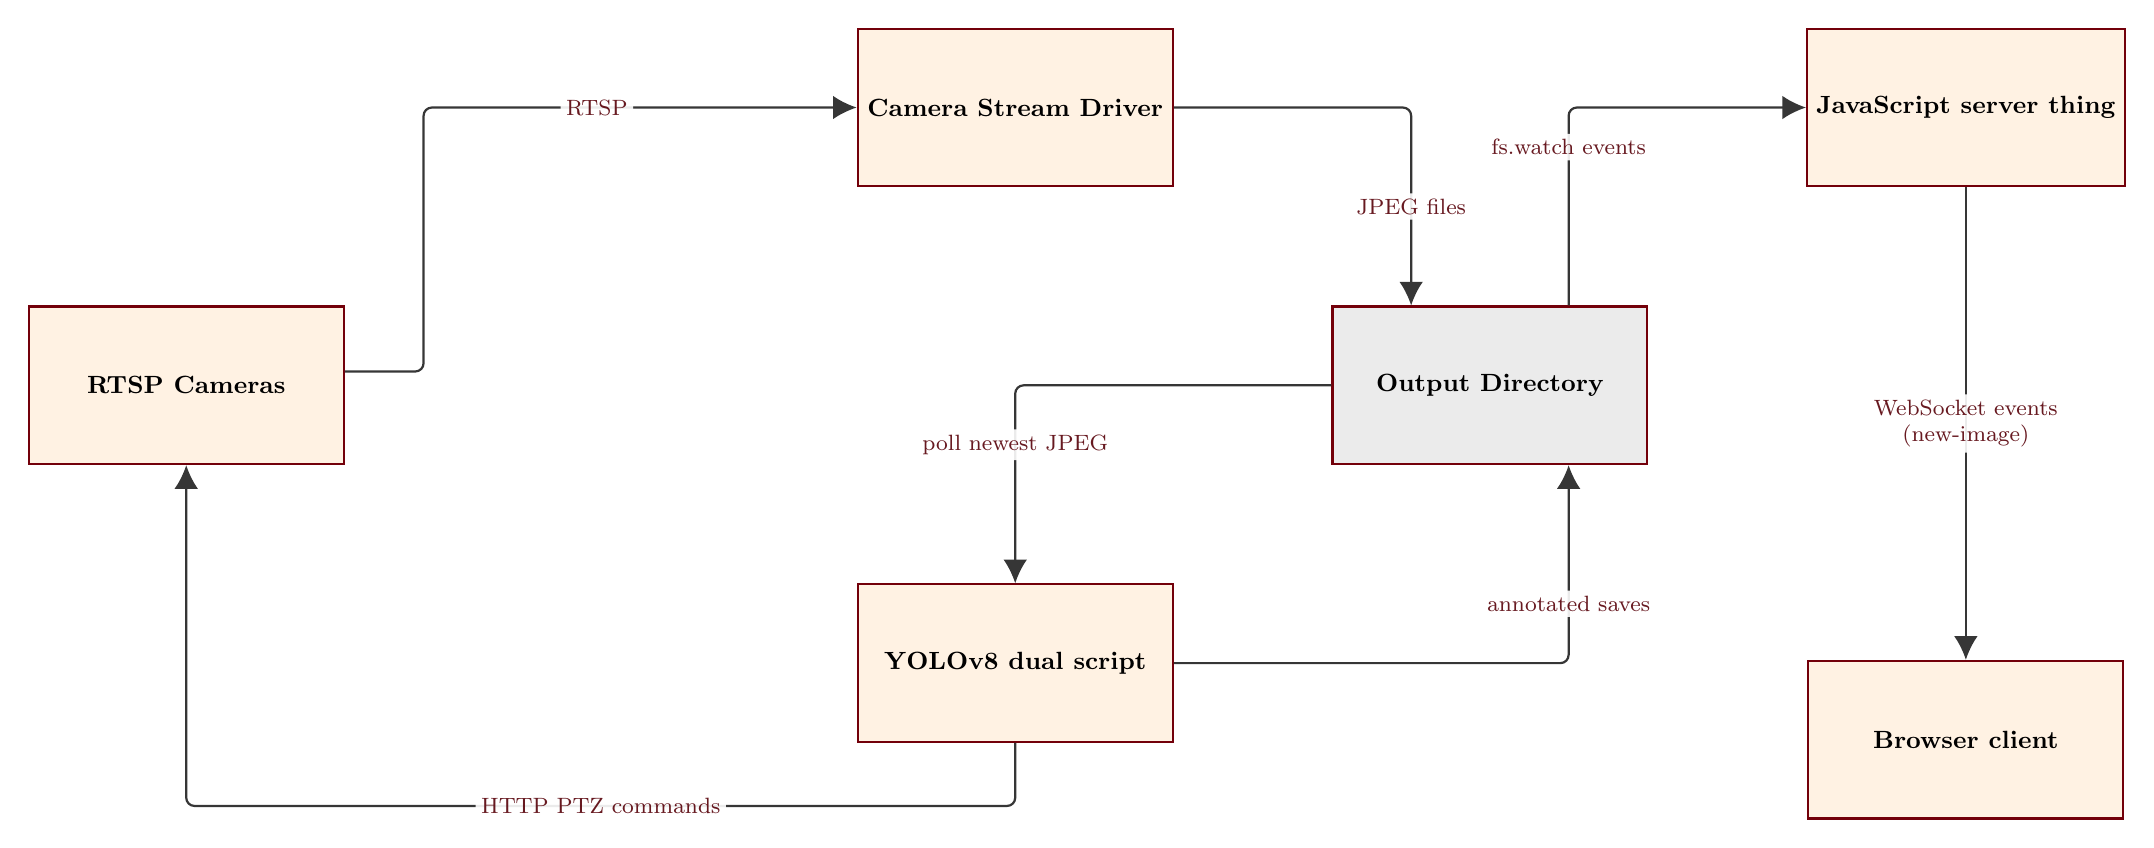
\begin{tikzpicture}[
    % Global Styles
    node distance=2cm and 2.5cm,
    block/.style={
        rectangle,
        draw=UofSCGarnet,      % Garnet Border
        thick,
        fill=UofSCSandstorm,   % Sandstorm Background
        text=UofSCBlack,       % Black Text
        align=center,
        minimum height=2cm,
        minimum width=4cm,
        font=\small\bfseries   % Bold text
    },
    arrow/.style={
        ->,
        >={Latex[width=3mm,length=3mm]},
        thick,
        draw=UofSC90Black,     % Dark Grey Arrows
        rounded corners=3pt
    },
    label_text/.style={
        fill=white,
        text=UofSCDarkGarnet,  % Dark Garnet for labels
        font=\footnotesize,
        align=center,
        inner sep=2pt,
        opacity=0.9
    }
]

    % --- Placement of Nodes ---
    
    % Center Node
    % Highlighting Output Directory slightly differently
    \node[block, fill=UofSC10Black] (output) {Output Directory};

    % Left Column
    \node[block, above left=1.5cm and 2cm of output] (driver) {Camera Stream Driver};
    \node[block, below left=1.5cm and 2cm of output] (yolo_rtsp) {YOLOv8 dual script};

    % Far Left (Source)
    % Align cam vertically between driver and yolo_rtsp
    \node[block, left=3.5cm of output, anchor=east] (cam) at ($(driver.west)!0.5!(yolo_rtsp.west) - (3cm, 0)$) {RTSP Cameras};

    % Right Column
    \node[block, above right=1.5cm and 2cm of output] (server) {JavaScript server thing};

    % Far Right (Client)
    \node[block, below=6cm of server] (client) {Browser client};


    % --- Connections with Offset Anchors to Prevent Crossing ---

    % 1. Cam -> Driver (Upper path)
    \draw[arrow] ([yshift=5pt]cam.east) -- ++(1,0) |- node[label_text, pos=0.7] {RTSP} (driver.west);

    % 2. Cam -> Yolo RTSP (Lower path)
    % \draw[arrow] ([yshift=-5pt]cam.east) -- ++(1,0) |- node[label_text, pos=0.7] {RTSP thread} (yolo_rtsp.west);
    
    % 3. Yolo RTSP -> Cam (Feedback Loop - Bottom)
    \draw[arrow] (yolo_rtsp.south) -- ++(0,-0.8) -| node[label_text, pos=0.25] {HTTP PTZ commands} (cam.south);

    % 4. Driver -> Output (Direct elbow)
    \draw[arrow] (driver.east) -| node[label_text, pos=0.75] {JPEG files} ([xshift=-1cm]output.north);

    % 5. Yolo RTSP -> Output (Direct elbow)
    \draw[arrow] (yolo_rtsp.east) -| node[label_text, pos=0.65] {annotated saves} ([xshift=1cm]output.south);

    % 6. Output -> Server (Direct elbow)
    \draw[arrow] ([xshift=1cm]output.north) |- node[label_text, pos=0.40] {fs.watch events} (server.west);

    % 7. Output -> Yolo JPEGS (Poll)
    \draw[arrow] (output.west) -| node[label_text, pos=0.65] {poll newest JPEG} (yolo_rtsp.north);
    
    % 9. Server -> Client
    \draw[arrow] (server.south) -- node[label_text] {WebSocket events\\(new-image)} (client.north);

\end{tikzpicture}%
}

\end{document}